% !TeX program = xelatex
\documentclass[a4paper,10pt]{article}

% ============================================================================
% កញ្ចប់បណ្ណាល័យ (Packages) – តាមលំនាំ NGS Preah Krasang (ls_plan.tex)
% បរិបទ៖ គ្មានស្លាយ LCD និងគ្មានម៉ាស៊ីនគិតលេខ — ប្រើសន្លឹកកិច្ចការសិស្ស (ស-ខ្មៅ) និងក្ដារខៀនជាគោល
% ============================================================================
\usepackage[a4paper, left=0.95cm, right=0.95cm, top=0.85cm, bottom=0.92cm, footskip=0.52cm]{geometry}
\usepackage{amsmath, amssymb}
\usepackage{unicode-math}
\usepackage{fontspec}
\usepackage{array, longtable, multirow, colortbl}
\usepackage[table]{xcolor}
\usepackage{enumitem}
\usepackage{pifont}
\usepackage{fancyhdr}
\usepackage{tikz}
\usetikzlibrary{calc, arrows.meta, angles, quotes, decorations.markings, decorations.pathreplacing, patterns, babel}

\makeatletter
\let\@expl@@@mark@update@singlecol@structures@@\relax
\makeatother

\providecommand{\NGSFindFonts}{%
  \IfFileExists{C:/Windows/Fonts/cambria.ttc}{%
    \def\NGSSysPath{C:/Windows/Fonts/}%
    \def\NGSUserPath{C:/Users/KIT/AppData/Local/Microsoft/Windows/Fonts/}%
  }{%
    \IfFileExists{./fonts/KhmerOSsiemreap.ttf}{\def\NGSSysPath{./fonts/}\def\NGSUserPath{./fonts/}}{%
    \IfFileExists{../fonts/KhmerOSsiemreap.ttf}{\def\NGSSysPath{../fonts/}\def\NGSUserPath{../fonts/}}{%
    \IfFileExists{../../fonts/KhmerOSsiemreap.ttf}{\def\NGSSysPath{../../fonts/}\def\NGSUserPath{../../fonts/}}{%
    \IfFileExists{../../../fonts/KhmerOSsiemreap.ttf}{\def\NGSSysPath{../../../fonts/}\def\NGSUserPath{../../../fonts/}}{%
    \IfFileExists{../../../../fonts/KhmerOSsiemreap.ttf}{\def\NGSSysPath{../../../../fonts/}\def\NGSUserPath{../../../../fonts/}}{%
    \IfFileExists{../../../../../fonts/KhmerOSsiemreap.ttf}{\def\NGSSysPath{../../../../../fonts/}\def\NGSUserPath{../../../../../fonts/}}{%
    \IfFileExists{../../../../../../fonts/KhmerOSsiemreap.ttf}{\def\NGSSysPath{../../../../../../fonts/}\def\NGSUserPath{../../../../../../fonts/}}{%
      \def\NGSSysPath{../../../../../../../fonts/}\def\NGSUserPath{../../../../../../../fonts/}%
    }}}}}}}%
  }%
}
\NGSFindFonts

\setmathfont[Path={\NGSSysPath}, FontIndex=1, Scale=1.02]{cambria.ttc}
\defaultfontfeatures{Ligatures=TeX}

\setmainfont[
  Path={\NGSUserPath}, Extension=.ttf, Script=Khmer,
  BoldFont={KhmerOSsiemreap}, BoldFeatures={FakeBold=1.8},
  ItalicFont={KhmerOSsiemreap}, ItalicFeatures={FakeSlant=0.25},
  BoldItalicFont={KhmerOSsiemreap}, BoldItalicFeatures={FakeBold=1.8, FakeSlant=0.25}
]{KhmerOSsiemreap}

\newfontfamily\muol[Path={\NGSUserPath}, Extension=.ttf, Script=Khmer]{KhmerOSmuollight}
\newfontfamily\TimesEn[Path={\NGSSysPath}, Extension=.ttf, Scale=1.00, BoldFont={timesbd}, ItalicFont={timesi}, BoldItalicFont={timesbi}]{times}
\newfontfamily\NagaBold[Path={\NGSUserPath}, Extension=.ttf]{AKbalthom Naga Bold}
\newfontfamily\CalibriFont[Path={\NGSSysPath}, Extension=.ttf]{calibri}
\newfontfamily\Tacteing[Path={\NGSUserPath}]{TACTENG.TTF}
\newfontfamily\CourierBullet[Path={\NGSSysPath}, Extension=.ttf]{cour}
\newcommand{\wcirc}{{\CourierBullet\fontsize{9.5pt}{11pt}\selectfont o}}

\XeTeXlinebreaklocale "km"
\XeTeXlinebreakskip = 0pt plus 1pt minus 0.1pt

\definecolor{stepgray}{HTML}{D9D9D9}
\definecolor{headgray}{HTML}{F2F2F2}
\definecolor{boxgray}{HTML}{D9D9D9}
\definecolor{darkred}{HTML}{C00000}
\definecolor{red5e}{HTML}{FF0000}

\pagestyle{fancy}
\fancyhf{}
\renewcommand{\headrulewidth}{0pt}
\fancyfoot[R]{\CalibriFont\fontsize{11pt}{13pt}\selectfont\thepage}

\setlength{\parindent}{0pt}
\setlength{\parskip}{0pt}
\setlength{\tabcolsep}{3.8pt}

\newcolumntype{L}[1]{>{\raggedright\arraybackslash}p{#1}}
\newcolumntype{C}[1]{>{\centering\arraybackslash}p{#1}}

\newcommand{\en}[1]{{\TimesEn #1}}
\newcommand{\enbf}[1]{{\TimesEn\textbf{#1}}}
\newcommand{\unit}[1]{\,\text{\en{#1}}}
\newcommand{\fiveE}[1]{{\NagaBold\fontsize{9.5pt}{13pt}\selectfont\textcolor{red5e}{#1}}}
\newcommand{\timenote}[1]{\textcolor{darkred}{\textit{#1}}}
\newcommand{\graybox}[1]{\colorbox{boxgray}{\strut\hspace{2pt}#1\hspace{2pt}}}
\newcommand{\cnum}[1]{{\fontsize{10.5pt}{12pt}\selectfont\ding{\numexpr181+#1\relax}}\hspace{0.15em}}
\newcommand{\cfig}[1]{\par\vspace{3pt}{\centering #1\par}\vspace{3pt}}
\newcommand{\stepheader}[1]{\multicolumn{3}{|c|}{\cellcolor{stepgray}\muol #1} \\* \noalign{\hrule height 0.4pt}}
\newcommand{\khmflourish}{{\Tacteing\fontsize{36pt}{14pt}\selectfont\raisebox{-5pt}{3}}}

% ============================================================================
% ម៉ាក្រូគូសរូប TikZ ស-ខ្មៅ ១០០% សម្រាប់មេរៀន ៥ ប្រមាណវិធីចែកចំនួនសនិទាន (RAT_DIV)
% ============================================================================

% ១. E1 Engage: បន្ទះវាស់ខ្សែបូ 4/5 m ចែកជាកំណាត់ 1/10 m (ឧទាហរណ៍ ក ទំ.១០)
\newcommand{\figEngageRATDIV}{%
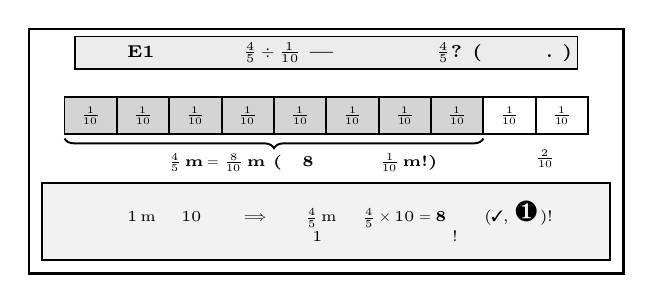
\begin{tikzpicture}[x=0.95cm, y=0.94cm, every node/.style={font=\scriptsize, text=black}]
  \draw[black, line width=0.95pt] (0,0) rectangle (7.95,3.30);
  \node[fill=gray!15, draw=black, line width=0.6pt, inner sep=2pt, font=\fontsize{6.2pt}{7.9pt}\selectfont\bfseries] at (3.975,2.98) {បេសកកម្ម \en{E1}៖ វាស់កាត់ខ្សែបូ $\frac{4}{5}\div\frac{1}{10}$ — ហេតុអ្វីផលចែកធំជាង $\frac{4}{5}$? (ឧទាហរណ៍ ក ទំ.១០)};

  % 10-cell ribbon bar from x=0.475 to 7.475 (width 0.70 each); shade 8 cells = 8/10 = 4/5
  \foreach \i in {0,...,7} {
    \fill[gray!34] (0.475+\i*0.70, 1.88) rectangle (0.475+\i*0.70+0.70, 2.38);
  }
  \foreach \i in {0,...,9} {
    \draw[black, line width=0.7pt] (0.475+\i*0.70, 1.88) rectangle (0.475+\i*0.70+0.70, 2.38);
    \node[font=\fontsize{5.2pt}{6.6pt}\selectfont] at (0.825+\i*0.70, 2.13) {$\frac{1}{10}$};
  }
  \draw[black, decorate, decoration={brace, mirror, amplitude=3.5pt}, line width=0.7pt] (0.475,1.82) -- (6.075,1.82);
  \node[font=\fontsize{5.4pt}{6.9pt}\selectfont\bfseries] at (3.275,1.50) {ប្រវែងខ្សែបូ $\frac{4}{5}\unit{m} = \frac{8}{10}\unit{m}$ (មាន $\mathbf{8}$ កំណាត់ប្រវែង $\frac{1}{10}\unit{m}$!)};
  \node[font=\fontsize{5.3pt}{6.8pt}\selectfont] at (6.775,1.55) {សល់ $\frac{2}{10}$};

  \draw[black, line width=0.75pt, fill=gray!10] (0.18,0.18) rectangle (7.77,1.22);
  \node[align=center, font=\fontsize{5.5pt}{7.2pt}\selectfont] at (3.975,0.70) {ក្នុង $1\unit{m}$ មាន $10$ កំណាត់ $\implies$ ក្នុង $\frac{4}{5}\unit{m}$ មាន $\frac{4}{5}\times 10 = \mathbf{8}$ កំណាត់ (\ding{51}, \cnum{1})!\\ពេលចែកនឹងប្រភាគសុទ្ធតូចជាង $1$ ផលចែកវិជ្ជមាន\textbf{ធំជាង}តំណាងចែកដើម!};
\end{tikzpicture}}

% ២. E2 POE 1 & POE 2: ក្បួនសោការពារតំណាងចែក [រក្សាទុក — គុណ — ច្រាស] និងសម្រួលខ្វែងក្រោយប្ដូរ
\newcommand{\figProtocolRATDIV}{%
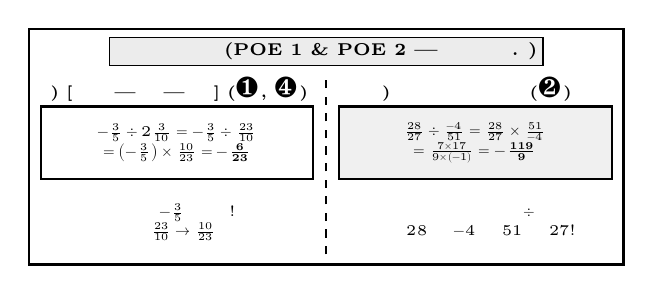
\begin{tikzpicture}[x=0.95cm, y=0.92cm, every node/.style={font=\scriptsize, text=black}]
  \draw[black, line width=0.95pt] (0,0) rectangle (7.95,3.25);
  \node[fill=gray!15, draw=black, line width=0.6pt, inner sep=2pt, font=\fontsize{6.2pt}{7.9pt}\selectfont\bfseries] at (3.975,2.94) {ក្បួនសោការពារតំណាងចែក \en{(POE 1 \& POE 2} — សៀវភៅពុម្ព ទំ.១០)};

  \draw[black, dashed, line width=0.65pt] (3.975,0.14) -- (3.975,2.62);

  % Left: Lock Dividend, Flip Divisor (ឧទាហរណ៍ ខ ទំ.១០)
  \node[font=\fontsize{5.6pt}{7.2pt}\selectfont\bfseries] at (1.98,2.42) {១) [រក្សាទុក — គុណ — ច្រាស] (\cnum{1}, \cnum{4})};
  \draw[black, line width=0.8pt] (0.16,1.18) rectangle (3.80,2.18);
  \node[align=center, font=\fontsize{5.4pt}{7.0pt}\selectfont] at (1.98,1.68) {$-\frac{3}{5} \div 2\frac{3}{10} = -\frac{3}{5} \div \frac{23}{10}$\\$= \left(-\frac{3}{5}\right) \times \frac{10}{23} = \mathbf{-\frac{6}{23}}$};
  \node[align=center, font=\fontsize{5.4pt}{6.9pt}\selectfont] at (1.98,0.58) {តំណាងចែក $-\frac{3}{5}$ \textbf{រក្សាដដែល}!\\ប្រែតែតួចែក $\frac{23}{10} \to \frac{10}{23}$ ប៉ុណ្ណោះ};

  % Right: Flip BEFORE cross-canceling (គំរូ ខ ទំ.១០)
  \node[font=\fontsize{5.6pt}{7.2pt}\selectfont\bfseries] at (5.96,2.42) {២) ប្ដូរជាគុណសិន ទើបសម្រួលខ្វែង (\cnum{2})};
  \draw[black, line width=0.8pt, fill=gray!12] (4.14,1.18) rectangle (7.79,2.18);
  \node[align=center, font=\fontsize{5.4pt}{7.0pt}\selectfont] at (5.965,1.68) {$\frac{28}{27} \div \frac{-4}{51} = \frac{28}{27} \times \frac{51}{-4}$\\$= \frac{7\times 17}{9\times (-1)} = \mathbf{-\frac{119}{9}}$};
  \node[align=center, font=\fontsize{5.4pt}{6.9pt}\selectfont] at (5.965,0.58) {\textbf{ហាម}សម្រួលខ្វែងពេលនៅសញ្ញា $\div$\\សម្រួល $28$ នឹង $-4$ និង $51$ នឹង $27$!};
\end{tikzpicture}}

% ៣. E4 Contrast Box: ចែកទសភាគរំកិលក្បៀស & អាទិភាពវង់ក្រចក (#9ឃ ទំ.១២)
\newcommand{\figBracketContrastRATDIV}{%
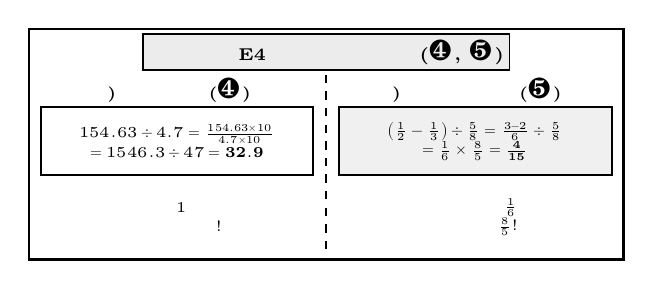
\begin{tikzpicture}[x=0.95cm, y=0.92cm, every node/.style={font=\scriptsize, text=black}]
  \draw[black, line width=0.95pt] (0,0) rectangle (7.95,3.18);
  \node[fill=gray!15, draw=black, line width=0.6pt, inner sep=2pt, font=\fontsize{6.2pt}{7.9pt}\selectfont\bfseries] at (3.975,2.86) {កាតពង្រីកចំណេះដឹង \en{E4}៖ ចែកទសភាគ និងអាទិភាពវង់ក្រចក (\cnum{4}, \cnum{5})};

  \draw[black, dashed, line width=0.65pt] (3.975,0.14) -- (3.975,2.54);

  \node[font=\fontsize{5.6pt}{7.2pt}\selectfont\bfseries] at (1.98,2.34) {១) បំបាត់ក្បៀសនៅតួចែក (\cnum{4})};
  \draw[black, line width=0.75pt] (0.16,1.16) rectangle (3.80,2.10);
  \node[align=center, font=\fontsize{5.5pt}{7.1pt}\selectfont] at (1.98,1.63) {$154.63 \div 4.7 = \frac{154.63\times 10}{4.7\times 10}$\\$= 1546.3 \div 47 = \mathbf{32.9}$};
  \node[align=center, font=\fontsize{5.4pt}{6.9pt}\selectfont] at (1.98,0.58) {រំកិលក្បៀសស្ដាំ $1$ ខ្ទង់ស្មើគ្នា\\រួចចែកដោយដៃតាមធម្មតា!};

  \node[font=\fontsize{5.6pt}{7.2pt}\selectfont\bfseries] at (5.96,2.34) {២) វង់ក្រចកមុនប្រមាណវិធីចែក (\cnum{5})};
  \draw[black, line width=0.8pt, fill=gray!12] (4.14,1.16) rectangle (7.79,2.10);
  \node[align=center, font=\fontsize{5.5pt}{7.1pt}\selectfont] at (5.965,1.63) {$\left(\frac{1}{2}-\frac{1}{3}\right)\div\frac{5}{8} = \frac{3-2}{6}\div\frac{5}{8}$\\$= \frac{1}{6}\times\frac{8}{5} = \mathbf{\frac{4}{15}}$};
  \node[align=center, font=\fontsize{5.4pt}{6.9pt}\selectfont] at (5.965,0.58) {គណនាក្នុងវង់ក្រចកបាន $\frac{1}{6}$ សិន\\ទើបគុណនឹងច្រាស $\frac{8}{5}$!};
\end{tikzpicture}}

% ៤. E5 Diagnostic Cards A-D
\newcommand{\figExitCardsRATDIV}{%
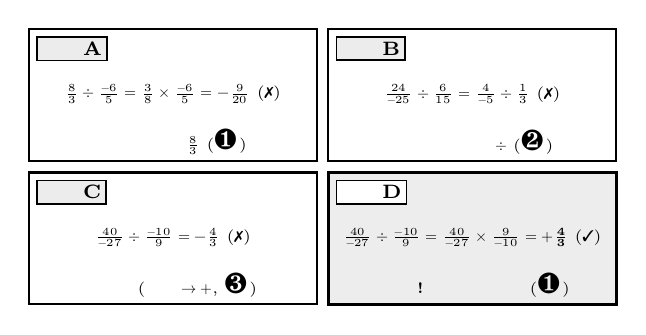
\begin{tikzpicture}[x=0.95cm, y=0.92cm, every node/.style={font=\scriptsize, text=black}]
  \draw[black, line width=0.9pt] (0,1.98) rectangle (3.85,3.80);
  \node[anchor=north west, fill=gray!15, draw=black, line width=0.6pt, inner sep=1.8pt] at (0.10,3.70) {\textbf{ជម្រើស \en{A}}};
  \node[font=\fontsize{5.6pt}{7.3pt}\selectfont] at (1.925,2.90) {$\frac{8}{3}\div\frac{-6}{5} = \frac{3}{8}\times\frac{-6}{5} = -\frac{9}{20}$ (\ding{55})};
  \node[font=\fontsize{5.5pt}{7.1pt}\selectfont] at (1.925,2.24) {ច្រឡំត្រឡប់តំណាងចែក $\frac{8}{3}$ (\cnum{1})};

  \draw[black, line width=0.9pt] (4.00,1.98) rectangle (7.85,3.80);
  \node[anchor=north west, fill=gray!15, draw=black, line width=0.6pt, inner sep=1.8pt] at (4.10,3.70) {\textbf{ជម្រើស \en{B}}};
  \node[font=\fontsize{5.6pt}{7.3pt}\selectfont] at (5.925,2.90) {$\frac{24}{-25}\div\frac{6}{15} = \frac{4}{-5}\div\frac{1}{3}$ (\ding{55})};
  \node[font=\fontsize{5.5pt}{7.1pt}\selectfont] at (5.925,2.24) {ច្រឡំសម្រួលខ្វែងលើសញ្ញា $\div$ (\cnum{2})};

  \draw[black, line width=0.9pt] (0,0) rectangle (3.85,1.82);
  \node[anchor=north west, fill=gray!15, draw=black, line width=0.6pt, inner sep=1.8pt] at (0.10,1.72) {\textbf{ជម្រើស \en{C}}};
  \node[font=\fontsize{5.6pt}{7.3pt}\selectfont] at (1.925,0.92) {$\frac{40}{-27}\div\frac{-10}{9} = -\frac{4}{3}$ (\ding{55})};
  \node[font=\fontsize{5.5pt}{7.1pt}\selectfont] at (1.925,0.26) {ច្រឡំសញ្ញា (ដកចែកដក $\to +$, \cnum{3})};

  \draw[black, line width=1.1pt, fill=gray!14] (4.00,0) rectangle (7.85,1.82);
  \node[anchor=north west, fill=white, draw=black, line width=0.6pt, inner sep=1.8pt] at (4.10,1.72) {\textbf{ជម្រើស \en{D}}};
  \node[font=\fontsize{5.6pt}{7.3pt}\selectfont] at (5.925,0.92) {$\frac{40}{-27}\div\frac{-10}{9} = \frac{40}{-27}\times\frac{9}{-10} = \mathbf{+\frac{4}{3}}$ (\ding{51})};
  \node[font=\fontsize{5.5pt}{7.1pt}\selectfont] at (5.925,0.26) {\textbf{ត្រឹមត្រូវ!} គុណនឹងច្រាស រួចសម្រួល (\cnum{1})};
\end{tikzpicture}}

\begin{document}
\fontsize{10pt}{15.2pt}\selectfont

% -------------------- ក្បាលកិច្ចតែងការ --------------------
\begin{center}
  {\muol\fontsize{11pt}{16pt}\selectfont ព្រះរាជាណាចក្រកម្ពុជា}\\[2pt]
  {\muol\fontsize{10pt}{15pt}\selectfont ជាតិ សាសនា ព្រះមហាក្សត្រ}\\[1pt]
  \khmflourish
\end{center}

\vspace{-24pt}
{\muol\fontsize{9.5pt}{12.5pt}\selectfont
មន្ទីរអប់រំ យុវជន និងកីឡា ខេត្តកំពង់ធំ\\
ការិយាល័យអប់រំ យុវជន និងកីឡា ស្រុកកំពង់ស្វាយ\\
អនុវិទ្យាល័យព្រះក្រសាំង}

\vspace{1pt}
\begin{center}
  {\muol\fontsize{10pt}{14pt}\selectfont កិច្ចតែងការបង្រៀន}
\end{center}
\vspace{0pt}

% -------------------- ព័ត៌មានទូទៅ --------------------
{\renewcommand{\arraystretch}{0.98}
\hspace*{3.1cm}%
\begin{tabular}{@{}l l L{11.0cm}@{}}
  - \hspace{0.35cm} មុខវិជ្ជា & : & គណិតវិទ្យា ថ្នាក់ទី៨ (ពីជគណិត) \\
  - \hspace{0.35cm} ចំណងជើងមេរៀន & : & មេរៀនទី១៖ ចំនួនសនិទាន \\
  - \hspace{0.35cm} ចំណងជើងរង & : & ៥. ប្រមាណវិធីចែកនៃចំនួនសនិទាន (ទំព័រ ១០ និងទំព័រ ១២) \\
  - \hspace{0.35cm} រយៈពេល & : & ១ ម៉ោងសិក្សា (៥០ នាទី) \\
  - \hspace{0.35cm} បង្រៀនដោយ & : & ហុក ប៊ុនថែន \\
  - \hspace{0.35cm} កាលបរិច្ឆេទ & : & ថ្ងៃសៅរ៍ ទី២១ ខែវិច្ឆិកា ឆ្នាំ២០២៦ \\
\end{tabular}

\vspace{2pt}

% -------------------- I. វត្ថុបំណង --------------------
\textbf{I.} {\muol វត្ថុបំណង}\\[1pt]
\hspace*{0.55cm}%
\begin{tabular}{@{}l l L{14.2cm}@{}}
  \wcirc \hspace{0.25cm} វិជ្ជាសម្បទា & : & សិស្សប្រាប់រូបមន្តចែកចំនួនសនិទាន ($\frac{a}{b}\div\frac{c}{d}=\frac{a}{b}\times\frac{d}{c}=\frac{ad}{bc}$ ចំពោះ $b,c,d\neq 0$) លក្ខខណ្ឌតួចែកមិនសូន្យ និងក្បួនសញ្ញានៃផលចែកបានត្រឹមត្រូវតាមសៀវភៅគោល (ទំ.១០) ។ \\
  \wcirc \hspace{0.25cm} បំណិនសម្បទា & : & សិស្សគណនាផលចែកប្រភាគមានសញ្ញា ចំនួនចម្រុះ ចំនួនទសភាគ និងកន្សោមមានវង់ក្រចកលើសន្លឹកកិច្ចការដោយដៃតាមក្បួន «រក្សាទុក-គុណ-ច្រាស» បានត្រឹមត្រូវ ។ \\
  \wcirc \hspace{0.25cm} ចរិយាសម្បទា & : & សិស្សមានទម្លាប់ប្រុងប្រយ័ត្ន ប្ដូរប្រមាណវិធីចែកជាវិធីគុណសិនមុនសម្រួលខ្វែង និងផ្ទៀងផ្ទាត់សញ្ញាផលចែកដោយហ្មត់ចត់ ។ \\
\end{tabular}

\vspace{2pt}

% -------------------- II. សម្ភារៈឧបទេស --------------------
\textbf{II.} {\muol សម្ភារៈឧបទេស}\\[1pt]
\hspace*{0.55cm}$\bullet$ \hspace{0.35cm} សៀវភៅសិក្សាគោលគណិតវិទ្យាថ្នាក់ទី៨ (ទំ.១០ និងទំ.១២) ក្ដារខៀន ដីស និងសន្លឹកកិច្ចការសិស្ស ស-ខ្មៅ (\en{Worksheet\_RAT\_DIV} ទំព័រ ១–២ គ្មានស្លាយ \en{LCD} គ្មានម៉ាស៊ីនគិតលេខ)

\vspace{2pt}

% -------------------- III. វិធីសាស្រ្តបង្រៀន --------------------
\textbf{III.} {\muol វិធីសាស្រ្តបង្រៀន}\\[1pt]
\hspace*{0.45cm}%
\begin{tabular}{@{}l l L{14.85cm}@{}}
  $\bullet$ \hspace{0.25cm} គោលវិធី & : & សិស្សមជ្ឈមណ្ឌល (បង្រៀនតាមសន្លឹកកិច្ចការស៊ើបអង្កេតជាដៃគូ និងក្ដារខៀន គ្មាន \en{LCD}) \\
  $\bullet$ \hspace{0.25cm} យុទ្ធវិធីបង្រៀន & : & គំរូ \en{5Es} រួមបញ្ចូលបន្ទះវាស់ខ្សែបូ សោការពារតំណាងចែក \en{(POE 1)} និងសម្រួលខ្វែងក្រោយប្ដូរ \en{(POE 2)} \\
\end{tabular}
}

\vspace{2pt}

% -------------------- IV. ដំណើរការបង្រៀន --------------------
\textbf{IV.} {\muol ដំណើរការបង្រៀន}

\vspace{1pt}

\renewcommand{\arraystretch}{1.15}
\begin{longtable}{|L{5.50cm}|L{7.90cm}|L{4.80cm}|}
\hline
\rowcolor{headgray}
\multicolumn{1}{|c|}{\muol សកម្មភាពគ្រូ} &
\multicolumn{1}{c|}{\muol ខ្លឹមសារមេរៀន} &
\multicolumn{1}{c|}{\muol សកម្មភាពសិស្ស} \\
\hline
\endfirsthead

\hline
\rowcolor{headgray}
\multicolumn{1}{|c|}{\muol សកម្មភាពគ្រូ} &
\multicolumn{1}{c|}{\muol ខ្លឹមសារមេរៀន} &
\multicolumn{1}{c|}{\muol សកម្មភាពសិស្ស} \\
\hline
\endhead

\hline
\endfoot

\hline
\endlastfoot

% ==================== ជំហានទី១ (2min) ====================
\stepheader{ជំហានទី១ \enbf{(}រដ្ឋបាលថ្នាក់\enbf{)}}
$\bullet$ ពិនិត្យអវត្តមាន អនាម័យ និងសណ្ដាប់ធ្នាប់ថ្នាក់រៀន \timenote{(2 min)}\par\vspace{2pt}
$\bullet$ ចែក \textbf{សន្លឹកកិច្ចការសិស្ស (\en{Worksheet\_RAT\_DIV})} ម្នាក់ ១ សន្លឹក (ផ្កាប់ទុកសិន)
&
$\bullet$ រដ្ឋបាលថ្នាក់ និងការរៀបចំដៃគូសិក្សា (២ នាក់ក្នុង ១ តុ)\par\vspace{2pt}
$\bullet$ សន្លឹកកិច្ចការសិស្ស ស-ខ្មៅ ២ ទំព័រ សម្រាប់បំពេញតាមជំហានមេរៀន
&
$\circ$ ប្រធានថ្នាក់រាយការណ៍អវត្តមាន\par\vspace{2pt}
$\circ$ ទទួលសន្លឹកកិច្ចការ ដាក់ផ្កាប់លើតុ \\[3pt]
\hline

% ==================== ជំហានទី២ (9min: <=3 + 3 + E1 3) ====================
\stepheader{ជំហានទី២ \enbf{(}កិច្ចការផ្ទះ \enbf{+} ទំនាក់ទំនងមេរៀនថ្មី\enbf{)}}
\timenote{កំណែកិច្ចការផ្ទះ ($\le 3\unit{min}$)}\par\vspace{2pt}
$\bullet$ ហៅសិស្ស ២ នាក់ឡើងកែកិច្ចការផ្ទះចំណុច ៤ (ទំ.១២ \#10ក,ខ,ឃ,ច) លើក្ដារខៀន
&
\textbf{១. កំណែកិច្ចការផ្ទះ (ប្រមាណវិធីគុណ និងលក្ខណៈ ទំ.១២ \#10)៖}\par\vspace{2pt}
$\bullet$ \textbf{១ក)} $-\dfrac{4}{5}\cdot\left(\dfrac{11}{17}\cdot\dfrac{10}{16}\right) = -\dfrac{11}{34}$ \;;\; \textbf{១ខ)} $-\left(\dfrac{11}{13}\cdot\dfrac{17}{16}\right)\cdot\dfrac{26}{51} = -\dfrac{11}{24}$\par\vspace{2pt}
$\bullet$ \textbf{២ក)} $\dfrac{21}{22}\left(-\dfrac{11}{8}+\dfrac{17}{16}\right) = -\dfrac{105}{352}$ \;;\; \textbf{២ខ)} $-\dfrac{11}{49}+\dfrac{33}{147} = 0$
&
$\circ$ តំណាងសិស្សឡើងកែលើក្ដារខៀន\par\vspace{2pt}
$\circ$ ផ្ទៀងផ្ទាត់ និងកែតម្រូវចូលសៀវភៅ \\[3pt]

\timenote{រំលឹកមេរៀនទាក់ទង (3 min)}\par\vspace{2pt}
$\bullet$ សួររំលឹកចំនួនច្រាស (ទំ.៩)៖ «តើចំនួនច្រាសនៃ $\frac{1}{10}$, $\frac{-6}{25}$ និង $2\frac{3}{10}$ គឺជាចំនួនណា? តើ $0$ មានចំនួនច្រាសឬទេ?»
&
\textbf{២. រំលឹកចំនួនច្រាស និងការបំប្លែងចំនួនចម្រុះ៖}\par\vspace{2pt}
$\bullet$ ច្រាសនៃ $\dfrac{1}{10}$ គឺ $\dfrac{10}{1}=10$ \;;\; ច្រាសនៃ $\dfrac{-6}{25}$ គឺ $\dfrac{25}{-6}=-\dfrac{25}{6}$
&
$\circ$ ឆ្លើយផ្ទាល់មាត់៖ $10$ និង $-\frac{25}{6}$ \\[3pt]

$\bullet$ បញ្ជាក់បន្ថែមលើចំនួនចម្រុះ និងលេខសូន្យ មុនភ្ជាប់ចូលប្រមាណវិធីចែក
&
$\bullet$ $2\dfrac{3}{10} = \dfrac{23}{10} \implies$ ចំនួនច្រាសគឺ $\dfrac{10}{23}$ \;;\; លេខ $0$ \textbf{គ្មាន}ចំនួនច្រាសទេ!
&
$\circ$ បំប្លែង $2\frac{3}{10}=\frac{23}{10}$ រួចប្រាប់ច្រាស $\frac{10}{23}$ \\[3pt]

\fiveE{E1 - Engage} \timenote{(3 min)}\par\vspace{2pt}
$\bullet$ ឱ្យសិស្សផ្ងារសន្លឹកកិច្ចការទំព័រទី១ អានបេសកកម្ម \en{E1} (ឧទាហរណ៍ ក ទំ.១០)៖ «ខ្សែបូប្រវែង $\frac{4}{5}\unit{m}$ ត្រូវកាត់ជាកំណាត់ប្រវែង $\frac{1}{10}\unit{m}$ ស្មើៗគ្នា ($\frac{4}{5}\div\frac{1}{10}$) ។ តើចំនួនកំណាត់ដែលបាន ធំជាង ឬតូចជាង $\frac{4}{5}$?»
&
\textbf{៣. បេសកកម្ម \en{E1} — បន្ទះវាស់ខ្សែបូ ($\frac{4}{5}\div\frac{1}{10}$)៖}\par\vspace{2pt}
$\bullet$ រាប់លើបន្ទះ $\frac{8}{10}\unit{m}$ ឃើញមាន $\mathbf{8}$ កំណាត់ ($\frac{4}{5}\div\frac{1}{10} = \frac{4}{5}\times\frac{10}{1} = 8$)!\par\vspace{2pt}
$\bullet$ ភ្ជាប់ចូលមេរៀនថ្មី៖ \textbf{៥. ប្រមាណវិធីចែកនៃចំនួនសនិទាន (ទំ.១០)}
&
$\circ$ គូសធីកការទស្សន៍ទាយ រាប់ក្រឡា $\frac{1}{10}$ លើបន្ទះខ្សែបូ ឃើញបាន $8$ កំណាត់! \\[3pt]

& \cfig{\figEngageRATDIV} & \\[3pt]
\hline

% ==================== ជំហានទី៣ (17min: E2 11 + E3 6) ====================
\stepheader{ជំហានទី៣ \enbf{(}ខ្លឹមសារមេរៀនថ្មី\enbf{)}}
\fiveE{E2 - Explore} \timenote{(11 min)}\par\vspace{2pt}
$\bullet$ សរសេរចំណងជើងមេរៀនលើក្ដារខៀន និងណែនាំ \textbf{សកម្មភាពទី១ (\en{POE 1} — សោការពារតំណាងចែក)} តាមឧទាហរណ៍ ក, ខ (ទំ.១០)
&
\textbf{៥. ប្រមាណវិធីចែកនៃចំនួនសនិទាន (ទំ.១០) — \en{POE 1}៖}\par\vspace{2pt}
$\bullet$ \textbf{ឧទាហរណ៍ ក (ទំ.១០)៖} $\dfrac{4}{5}\div\dfrac{1}{10} = \dfrac{4}{5}\times\dfrac{10}{1} = \dfrac{40}{5} = \graybox{$8$}$
&
$\circ$ កត់ចំណងជើងមេរៀន និងគូសប្រអប់សោការពារតំណាងចែកលើសន្លឹកកិច្ចការ \\[3pt]

$\bullet$ ឱ្យដៃគូសាកល្បង \textbf{ឧទាហរណ៍ ខ} (ទំ.១០) និងឆ្លើយសំណួរអន្ទាក់៖ «បើច្រឡំត្រឡប់ប្រភាគទី១ $-\frac{5}{3}\times\frac{23}{10}$ តើខុសយ៉ាងដូចម្ដេច?»
&
$\bullet$ \textbf{ឧទាហរណ៍ ខ (ទំ.១០)៖} $-\dfrac{3}{5}\div 2\dfrac{3}{10} = -\dfrac{3}{5}\div\dfrac{23}{10} = -\dfrac{3}{5}\times\dfrac{10}{23} = \graybox{$-\dfrac{6}{23}$}$
&
$\circ$ បំប្លែង $2\frac{3}{10}=\frac{23}{10}$ រក្សាទុក $-\frac{3}{5}$ រួចគុណនឹងច្រាស $\frac{10}{23}$ \\[3pt]

$\bullet$ ណែនាំ \textbf{សកម្មភាពទី២ (\en{POE 2} — សម្រួលខ្វែងក្រោយប្ដូរជាគុណ)} លើ \textbf{លំហាត់គំរូ ក, ខ} (ទំ.១០)៖\par\vspace{2pt}
\hspace*{0.3em}-- \textbf{ទស្សន៍ទាយ (\en{P})៖} «ក្នុង $\frac{24}{-25}\div\frac{6}{15}$ តើអាចសម្រួល $24$ នឹង $15$ ភ្លាម ឬត្រូវប្ដូរជាគុណសិន?»
&
\textbf{សម្រួលខ្វែងក្រោយប្ដូរជាគុណ (ទំ.១០) — \en{POE 2}៖}\par\vspace{2pt}
$\bullet$ \textbf{គំរូ ក៖} $\dfrac{24}{-25}\div\dfrac{6}{15} = \dfrac{24}{-25}\times\dfrac{15}{6} = \dfrac{4\times 3}{-5} = \graybox{$-\dfrac{12}{5}$}$\par\vspace{2pt}
$\bullet$ \textbf{គំរូ ខ៖} $\dfrac{28}{27}\div\dfrac{-4}{51} = \dfrac{28}{27}\times\dfrac{51}{-4} = \dfrac{7\times 17}{-9} = \graybox{$-\dfrac{119}{9}$}$
&
$\circ$ រកឃើញថាត្រូវប្ដូរ $\div$ ជា $\times$ និងត្រឡប់តួចែកសិន ទើបសម្រួលខ្វែងបានត្រឹមត្រូវ! \\[3pt]

& \cfig{\figProtocolRATDIV} & \\[3pt]

\fiveE{E3 - Explain} \timenote{(6 min)}\par\vspace{2pt}
$\bullet$ ហៅតំណាងដៃគូឡើងបង្គុំរូបមន្តប្រអប់ «ជាទូទៅ» នៃប្រមាណវិធីចែកចំនួនសនិទាន (ទំ.១០)
&
\textbf{សំយោគបញ្ញត្តិ និងធនាគារហេតុផល \en{B\&W} (\cnum{1}--\cnum{5})៖}\par\vspace{2pt}
$\bullet$ \textbf{ជាទូទៅ (ទំ.១០)៖} ចំពោះ $b\neq 0,\; c\neq 0,\; d\neq 0$ គេបាន៖\par\vspace{1.5pt}
$\dfrac{a}{b}\div\dfrac{c}{d} = \dfrac{a}{b}\times\dfrac{d}{c} = \dfrac{ad}{bc}$ \quad (ហាមចែកនឹង $0$ ដាច់ខាត!)
&
$\circ$ កត់ត្រារូបមន្តប្រអប់ «ជាទូទៅ» និងលក្ខខណ្ឌ $b,c,d\neq 0$ លើសន្លឹកកិច្ចការ \\[3pt]

$\bullet$ បញ្ជាក់ថាប្រមាណវិធីចែក\textbf{គ្មាន}លក្ខណៈត្រឡប់ ឬផ្គុំទេ រួចសង្ខេបធនាគារហេតុផល \cnum{1}--\cnum{3}
&
\cnum{1} ក្បួន ៣ ពាក្យ \textbf{[រក្សាទុក — គុណ — ច្រាស]}៖ $\frac{a}{b}\div\frac{c}{d}=\frac{a}{b}\times\frac{d}{c}$ ។\par\vspace{1.5pt}
\cnum{2} \textbf{ហាម}សម្រួលខ្វែងពេលនៅសញ្ញា $\div$ ត្រូវប្ដូរជាវិធីគុណសិនទើបសម្រួល ។\par\vspace{1.5pt}
\cnum{3} ក្បួនសញ្ញាផលចែកដូចវិធីគុណ៖ ដូចគ្នា $\to +$ ; ផ្ទុយគ្នា $\to -$ ។
&
$\circ$ ផ្ទៀងផ្ទាត់ហេតុផល \cnum{1}--\cnum{3} លើសន្លឹកកិច្ចការ \\[3pt]

$\bullet$ បន្ថែមហេតុផល \cnum{4}--\cnum{5} សម្រាប់ចំនួនចម្រុះ ទសភាគ និងអាទិភាពវង់ក្រចក
&
\cnum{4} បំប្លែងចំនួនចម្រុះជាប្រភាគសិន ឬរំកិលក្បៀសបំបាត់ទសភាគនៅតួចែក ។\par\vspace{1.5pt}
\cnum{5} អាទិភាពប្រមាណវិធី៖ គណនាក្នុងវង់ក្រចកសិន មុនធ្វើប្រមាណវិធីចែក ។
&
$\circ$ ធ្វើលំហាត់ត្រួតពិនិត្យរហ័សនៅបាតទំព័រទី១ \\[3pt]
\hline

% ==================== ជំហានទី៤ (20min: E4 10 + E5 10) ====================
\stepheader{ជំហានទី៤ \enbf{(}ពង្រឹង និងពង្រីកចំណេះដឹង\enbf{)}}
\fiveE{E4 - Elaborate} \timenote{(10 min)}\par\vspace{2pt}
$\bullet$ ឱ្យសិស្សបើកសន្លឹកកិច្ចការទំព័រទី២ (ផ្នែកទី៣) គណនា \textbf{លំហាត់គំរូ គ} (ទំ.១០) និងចែកទសភាគ
&
\textbf{១. លំហាត់គំរូ គ (ទំ.១០) ចែកទសភាគ និងកន្សោមវង់ក្រចក (ទំ.១២)៖}\par\vspace{2pt}
$\bullet$ \textbf{គំរូ គ (ទំ.១០)៖} $\dfrac{-18}{65}\div\dfrac{-6}{25} = \dfrac{-18}{65}\times\dfrac{25}{-6} = \dfrac{3\times 5}{13\times 1} = \graybox{$\dfrac{15}{13}$} \quad (\text{\cnum{1}, \cnum{3}})$\par\vspace{2pt}
$\bullet$ \textbf{ចែកទសភាគ៖} $14.4\div(-0.12) = 1440\div(-12) = \graybox{$-120$} \quad (\text{\cnum{4}})$
&
$\circ$ បំពេញជំហានគណនាដោយដៃ និងរំកិលក្បៀសបំបាត់ទសភាគនៅតួចែក \\[3pt]

$\bullet$ ដឹកនាំលំហាត់កន្សោមវង់ក្រចក (ទំ.១២ \#9ឃ) និងសំណួរឆ្លុះបញ្ចាំង \en{EIA Looking-Back}
&
$\bullet$ \textbf{ទំ.១២ \#9ឃ៖} $\left(\dfrac{1}{2}-\dfrac{1}{3}\right)\div\dfrac{5}{8} = \dfrac{3-2}{6}\div\dfrac{5}{8} = \dfrac{1}{6}\times\dfrac{8}{5} = \graybox{$\dfrac{4}{15}$} \quad (\text{\cnum{5}})$\par\vspace{3pt}
&
$\circ$ ឆ្លើយសំណួរ \en{EIA Looking-Back} ស្ដីពីអន្ទាក់ចែកមិនមានលក្ខណៈត្រឡប់ \\[4pt]

& \cfig{\figBracketContrastRATDIV} & \\[3pt]

\fiveE{E5 - Evaluate} \timenote{(10 min)}\par\vspace{2pt}
$\bullet$ ឱ្យសិស្សធ្វើលំហាត់ \textbf{ប្រតិបត្តិ ក, ខ} (ទំ.១០) លើសន្លឹកកិច្ចការ រួចប្ដូរសន្លឹកផ្ទៀងផ្ទាត់ជាដៃគូ (\en{Pause-Review})
&
\textbf{២. ប្រតិបត្តិ (សៀវភៅពុម្ព ទំ.១០)៖}\par\vspace{2pt}
$\bullet$ \textbf{ក)} $\dfrac{8}{3}\div\dfrac{-6}{5} = \dfrac{8}{3}\times\dfrac{5}{-6} = \mathbf{-\dfrac{20}{9}}$ \;;\; \textbf{ខ)} $\dfrac{40}{-27}\div\dfrac{-10}{9} = \dfrac{40}{-27}\times\dfrac{9}{-10} = \mathbf{\dfrac{4}{3}}$
&
$\circ$ គណនាប្រតិបត្តិ ក, ខ ដោយដៃ និងផ្ទៀងផ្ទាត់សញ្ញាជាដៃគូ \\[4pt]

$\bullet$ បន្តផ្ទៀងផ្ទាត់ \textbf{ប្រតិបត្តិ គ} (ចែកទសភាគ ទំ.១០) និងបិទបញ្ចប់បេសកកម្ម \en{E1}
&
$\bullet$ \textbf{គ)} $154.63\div 4.7 = 1546.3\div 47 = \mathbf{32.9}$\par\vspace{2pt}
$\bullet$ \textbf{បិទ \en{E1}៖} $\dfrac{4}{5}\div\dfrac{1}{10} = \dfrac{4}{5}\times 10 = \mathbf{8}$ កំណាត់ខ្សែបូ \mbox{(\cnum{1})!}
&
$\circ$ រំកិលក្បៀសចែកទសភាគ និងបិទបញ្ចប់បេសកកម្ម \en{E1} \\[4pt]

$\bullet$ វាយតម្លៃរហ័ស \textbf{៦០ វិនាទី}៖ ឱ្យសិស្សគូសវង់ជម្រើសត្រឹមត្រូវក្នុងប្រអប់ \en{A--D} និងបំពេញសំបុត្រចេញ
&
\textbf{៣. វិនិច្ឆ័យកំហុសរហ័ស (\en{A--D})៖} ចម្លើយត្រឹមត្រូវគឺ \graybox{\textbf{ជម្រើស \en{D}}} ($+\frac{4}{3}$) ។\par\vspace{2pt}
(\en{A} ច្រឡំត្រឡប់តំណាងចែក; \en{B} សម្រួលខ្វែងលើ $\div$; \en{C} ច្រឡំសញ្ញាដកចែកដក)
&
$\circ$ គូសវង់ជម្រើស \en{D} និងបំពេញសំបុត្រចេញមុនបញ្ចប់ម៉ោង \\[3pt]

& \cfig{\figExitCardsRATDIV} & \\[3pt]
\hline

% ==================== ជំហានទី៥ (<=2min) ====================
\stepheader{ជំហានទី៥ \enbf{(}កិច្ចការផ្ទះ \enbf{+} បណ្ដាំផ្ញើ\enbf{)}}
\timenote{ចំណាយពេលឱ្យតិចបំផុតកុំឱ្យលើស 2 min}\par\vspace{2pt}
$\bullet$ ណែនាំកិច្ចការផ្ទះនៅផ្នែកទី៥ នៃសន្លឹកកិច្ចការ (ទំ.១២ \#9ង និងបុរេសិក្សាចំណោទ ទំ.១០) និងផ្ដាំផ្ញើឱ្យអានមុនចំណុច \textbf{៦. ចំណោទ} (ទំ.១០–១២)
&
\centerline{\muol កិច្ចការផ្ទះ}\par\vspace{2pt}
$\bullet$ \textbf{លំហាត់ ១៖} គណនា រួចសម្រួល៖ ក) $-\dfrac{15}{28}\div\dfrac{5}{-14}$ \quad ខ) $\left(\dfrac{1}{2}+\dfrac{1}{3}\right)\div\left(\dfrac{5}{8}-\dfrac{1}{4}\right)$ (ទំ.១២ \#9ង)\par\vspace{2pt}
$\bullet$ \textbf{លំហាត់ ២ (ភ្ជាប់ចំណោទ ទំ.១០)៖} ចតុកោណកែងមួយមានបរិមាត្រ $16.38\unit{cm}$ ។ រកកន្លះបរិមាត្រ $p = 16.38\div 2$ ។\par\vspace{2pt}
$\bullet$ \textbf{បណ្ដាំផ្ញើ៖} អានមុនចំណុច \textbf{៦. ចំណោទ} និងលំហាត់សំយោគមេរៀនទី១ (ទំ.១០–១២) ។
&
$\circ$ កត់ត្រាកិច្ចការផ្ទះ និងទទួលបណ្ដាំផ្ញើដោយសណ្ដាប់ធ្នាប់ \\[3pt]
\end{longtable}

% -------------------- កាលបរិច្ឆេទ និងហត្ថលេខា --------------------
\vspace{2pt}
\hfill
\begin{minipage}{9.8cm}
  {\centering
    ថ្ងៃសៅរ៍ ១២កើត ខែកត្តិក ឆ្នាំមមី អដ្ឋស័ក ពុទ្ធសករាជ ២៥៧០\\[2pt]
    ត្រូវនឹងថ្ងៃទី២១ ខែវិច្ឆិកា ឆ្នាំ២០២៦\\[3pt]
    {\muol គ្រូបង្រៀន}\par}
  \vspace{28pt}
  \hfill{\muol ហុក ប៊ុនថែន}\hspace*{1.4cm}
\end{minipage}

\end{document}
